\chapter{Property-Based Testing in a Screencast Editor: Introduction - Oskar Wickstr\"om}
\label{sec:screencast_introduction}


\begin{quotation}
\noindent\textit{\textbf{William Yao:}}
\textit{Probably the best series of posts I've read about using property-based testing in practice. Lots of interesting tricks and techniques explored. Highly recommended.}

\vspace{\baselineskip}
\noindent\textit{Original article: \cite{screencast_introduction}}
\end{quotation}
This is the first in a series of posts about using property-based testing (PBT) within \textit{Komposition}, a screencast editor that I've been working on during the last year. It introduces PBT and highlights some challenges in testing properties of an application like Komposition.

Future posts will focus on individual case studies, covering increasingly complex components and how they are tested. I'll reflect on what I've learned in each case, what bugs the tests have found, and what still remains to be improved.

For example, I'll explain how using PBT helped me find and fix bugs in the specification and implementation of Komposition's video classifier. Those were bugs that would be very hard to find using example-based tests or using a static type system!

This series is not a tutorial on PBT, but rather a collection of motivating examples. That said, you should be able to follow along without prior knowledge of PBT.

\section{Komposition}


In early 2018 I started producing \href{https://haskell-at-work.com/}{Haskell screencasts}. A majority of the work involved cutting and splicing video by hand in a \href{https://en.wikipedia.org/wiki/Non-linear_editing_system}{non-linear editing system (NLE)} like \href{https://en.wikipedia.org/wiki/Adobe_Premiere_Pro}{Premiere Pro} or \href{https://kdenlive.org/en/}{Kdenlive}. I decided to write a screencast editor specialized for my needs, reducing the amount of manual labor needed to edit the recorded material. Komposition was born.

Komposition is a modal GUI application built for editing screencasts. Unlike most NLE systems, it features a hierarchical timeline, built out of \textit{sequences}, \textit{parallels}, \textit{tracks}, \textit{clips} and \textit{gaps}. To make the editing experience more efficient, it automatically classifies scenes in screen capture video, and sentences in recorded voice-over audio.

If you are curious about Komposition and want to learn more right away, check out its \href{https://owickstrom.github.io/komposition/}{documentation}.
\begin{figure}[htbp]
 \centering
 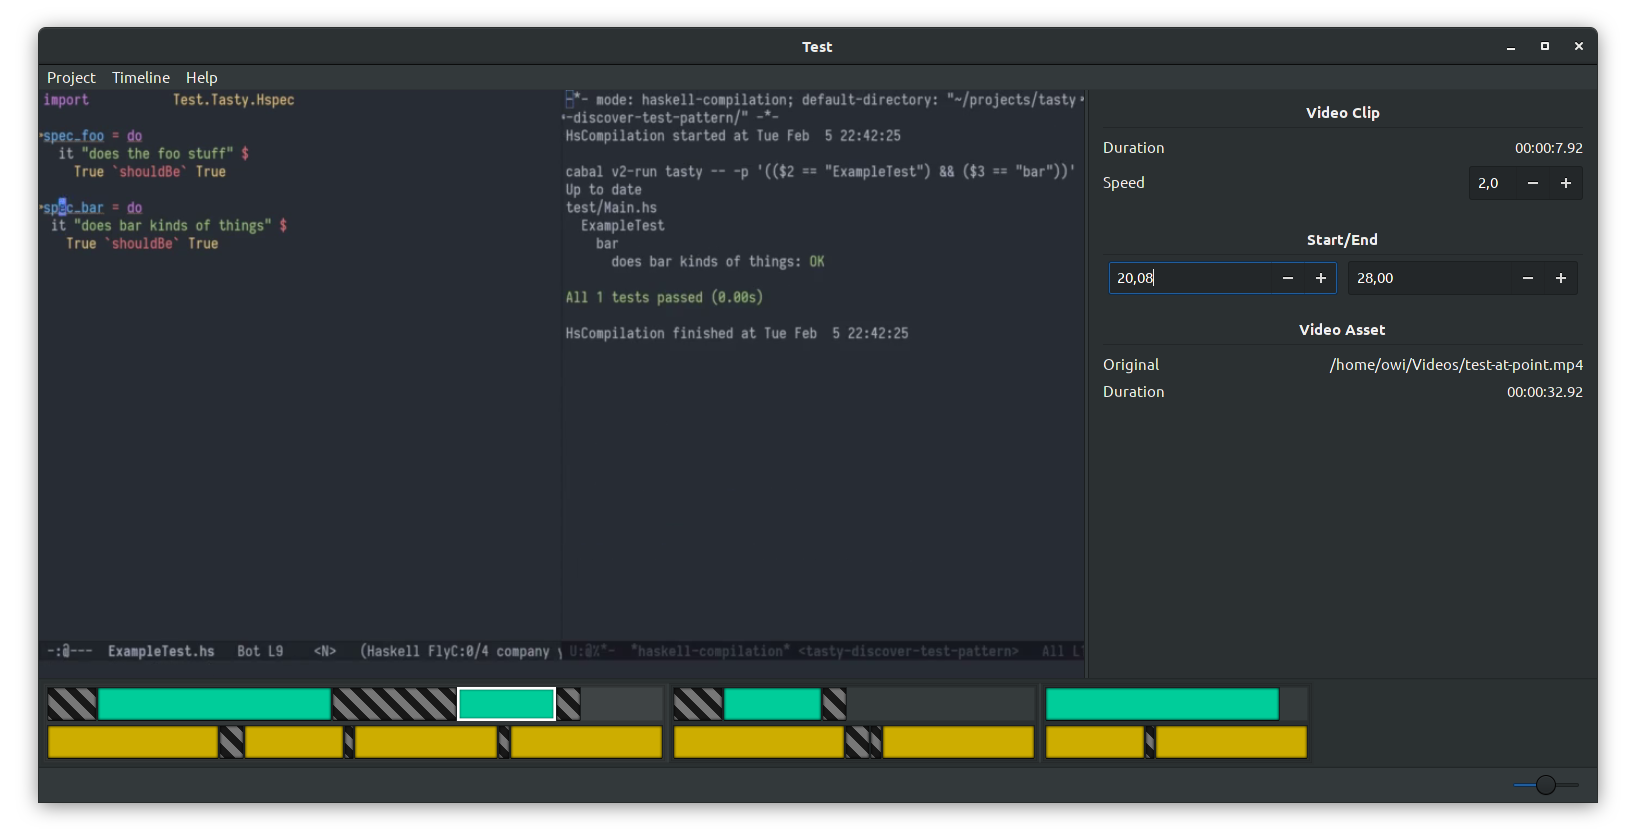
\includegraphics[width=.95\linewidth]{./pics/komposition-light.png}
 \caption{Komposition's timeline mode}
 \label{fig:komposition_time_line_mode}
\end{figure}
Some of the most complex parts of Komposition include focus and timeline transformations, video classification, video rendering, and the main application logic. Those are the areas in which I've spent most effort writing tests, using a combination of example-based and property-based testing.

I've selected the four most interesting areas where I've applied PBT in Komposition, and I'll cover one in each coming blog post:

\begin{enumerate}
\item Timeline flattening
\item Video scene classification
\item Focus and timeline consistency
\item Symmetry of undo/redo
\end{enumerate}
I hope these case studies will be motivating, and that they will show the value of properties all the way from unit testing to integration testing.

\section{Property-Based Testing}


To get the most out of this series, you need a basic understanding of what PBT is, so let's start there. For my take on a minimal definition, PBT is about:

\begin{enumerate}
\item Specifying your system under test in terms of properties, where properties describe invariants of the system based on its input and output.
\item Testing that those properties hold against a large variety of inputs.
\end{enumerate}
It's worth noting that PBT is not equal to QuickCheck, or any other specific tool, for that matter. The set of inputs doesn't have to be randomly generated. You don't have to use ``shrinking''. You don't have to use a static type system or a functional programming language. PBT is a general idea that can be applied in many ways.

The following resources are useful if you want to learn more about PBT:

\begin{itemize}
\item The \href{https://hypothesis.works/articles/intro/}{introductory articles on Hypothesis}, although specific to Python.
\item \href{https://hypothesis.works/articles/what-is-property-based-testing/}{``What is Property Based Testing?''} by David R. MacIver is a definition of what PBT is, and particularly what it isn't.
\end{itemize}
The code examples will be written in Haskell and using the \href{https://hackage.haskell.org/package/hedgehog}{Hedgehog} testing system. You don't have to know Haskell to follow this series, as I'll explain the techniques primarily without code. But if you are interested in the Haskell specifics and in Hedgehog, check out \href{https://teh.id.au/posts/2017/04/23/property-testing-with-hedgehog/}{``Property testing with Hedgehog''} by Tim Humphries.

\section{Properties of the Ugly Parts}


When I started with PBT, I struggled with applying it to anything beyond simple functions. Examples online are often focused on the fundamentals. They cover concepts like reversing lists, algebraic laws, and symmetric encoders and decoders. Those are important properties to test, and they are good examples for teaching the foundations of PBT.

I wanted to take PBT beyond pure and simple functions, and leverage it on larger parts of my system. The ``ugly'' parts, if you will. In my experience, the complexity of a system often becomes much higher than the sum of its parts. The way subsystems are connected and form a larger graph of dependencies drives the need for integration testing at an application level.

Finding resources on integration testing using PBT is hard, and it might drive you to think that PBT is not suited for anything beyond the introductory examples. With the case studies in this blog series I hope to contribute to debunking such misconceptions.

\section{Designing for Testability}


In my case, it's a desktop multimedia application. What if we're working on a backend that connects to external systems and databases? Or if we're writing a frontend application with a GUI driven by user input? In addition to these kinds of systems being hard to test at a high level due to their many connected subsystems, they usually have stateful components, side effects, and non-determinism. How do we make such systems testable with properties?

Well, the same way we would design our systems to be testable with examples. Going back to \href{https://testing.googleblog.com/2008/08/by-miko-hevery-so-you-decided-to.html}{``Writing Testable Code''} by Mi\v{s}ko Hevery from 2008, and Kent Beck's \href{https://www.amazon.com/Test-Driven-Development-Kent-Beck/dp/0321146530}{``Test-Driven Development by Example''} from 2003, setting aside the OOP specifics, many of their guidelines apply equally well to code tested with properties:

\begin{description}
\item[Determinism:] Make it possible to run the ``system under test'' deterministically, such that your tests can be reliable. This does not mean the code has to be pure, but you might need to stub or otherwise control side effects during your tests.
\item[No global state:] In order for tests to be repeatable and independent of execution order, you might have to rollback database transactions, use temporary directories for generated files, stub out effects, etc.
\item[High cohesion:] Strive for modules of high cohesion, with smaller units each having a single responsibility. Spreading closely related responsibilities thin across multiple modules makes the implementation harder to maintain and test.
\item[Low coupling:] Decrease coupling between interface and implementation. This makes it easier to write tests that don't depend on implementation details. You may then modify the implementation without modifying the corresponding tests.
\end{description}I find these guidelines universal for writing testable code in any programming language I've used professionally, regardless of paradigm or type system. They apply to both example-based and property-based testing.

\section{Patterns for Properties}


Great, so we know how to write testable code. But how do we write properties for more complex units, and even for integration testing? There's not a lot of educational resources on this subject that I know of, but I can recommend the following starting points:

\begin{itemize}
\item \href{https://fsharpforfunandprofit.com/posts/property-based-testing-2/}{``Choosing properties for property-based testing''} by Scott Wlaschin, giving examples of properties within a set of common categories.
\item The talk \href{https://www.youtube.com/watch?v=shngiiBfD80}{``Property-Based Testing for Better Code''} by Jessica Kerr, with examples of generating valid inputs and dealing with timeouts.
\end{itemize}
Taking a step back, we might ask ``Why it's so hard to come up with these properties?'' I'd argue that it's because doing so forces us to understand our system in a way we're not used to. It's challenging understanding and expressing the general behavior of a system, rather than particular \textit{anecdotes} that we've observed or come up with.

If you want to get better at writing properties, the only advice I can give you (in addition to studying whatever you can find in other projects) is to \textit{practice}. Try it out on whatever you're working on. Talk to your colleagues about using properties in addition to example-based tests at work. Begin at a smaller scale, testing simple functions, and progress towards testing larger parts of your system once you're comfortable. It's a long journey, filled with reward, surprise, and joy!

\section{Testing Case Studies}


With a basic understanding of PBT, how we can write testable code, and how to write properties for our system under test, we're getting ready to dive into the case studies:

\begin{enumerate}
\item Introduction (this chapter)
\item Timeline Flattening (see chapter \ref{sec:timeline_flattening})
\item Video Scene Classification (see chapter \ref{sec:video_scene_classification})
\item Integration Testing (see chapter \ref{sec:integration_testing})
\end{enumerate}


\section{Credits}

Thank you Chris Ford, Alejandro Serrano Mena, Tobias Pflug, Hillel Wayne, and Ulrik Sandberg for kindly providing your feedback on my drafts!


\chapter{Case Study 1: Timeline Flattening - Oskar Wickstr\"om}
\label{sec:timeline_flattening}

\vspace{\baselineskip}
\noindent\textit{Original article: \cite{timeline_flattening}}
\vspace{\baselineskip}

\noindent In the first post of this series I introduced the Komposition screencast editor, and briefly explained the fundamentals of property-based testing (PBT). Furthermore, I covered how to write testable code, regardless of how you check your code with automated tests. Lastly, I highlighted some difficulties in using properties to perform component and integration testing.

If you haven't read the introductory post, I suggest doing so before continuing with this one. You'll need an understanding of what PBT is for this case study to make sense.

This post is the first case study in the series, covering the timeline flattening process in Komposition and how it's tested using PBT. The property tests aren't integration-level tests, but rather unit tests. This case study serves as a warm-up to the coming, more advanced, ones.

Before we look at the tests, we need to learn more about Komposition's hierarchical timeline and how the flattening process works.

\section{The Hierarchical Timeline}

Komposition's timeline is hierarchical. While many non-linear editing systems have support for some form of nesting\footnote{Final Cut Pro has \href{https://support.apple.com/kb/PH12631?locale=en_US}{compound clips}, and Adobe Premiere Pro has \href{https://www.premiumbeat.com/blog/nesting-in-adobe-premiere-pro/}{nested sequences}}. they are primarily focused on flat timeline workflows. The timeline structure and the keyboard-driven editing in Komposition is optimized for the screencast editing workflow I use.

It's worth emphasizing that Komposition is not a general video editor. In addition to its specific editing workflow, you may need to adjust your recording workflow to use it effectively\footnote{The section on \href{https://owickstrom.github.io/komposition/user-guide/workflow/}{workflow} in Komposition's documentation describes how to plan, record, and edit your screencast in way compatible with Komposition.}.

\subsection{Video and Audio in Parallels}

At the lowest level of the timeline are \textit{clips} and \textit{gaps}. Those are put within the video and audio \textit{tracks of parallels}. The following diagram (figuare \ref{fig:case1_1}) shows a parallel consisting of two video clips and one audio clip.
\begin{figure}[htbp]
 \centering
 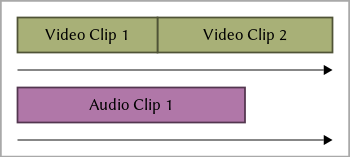
\includegraphics[width=.95\linewidth]{./pics/case1_1.png}
 \caption{Clips and gaps are placed in video and audio tracks}
 \label{fig:case1_1}
\end{figure}
The tracks of a parallel are played simultaneously (in parallel), as indicated by the arrows in the above diagram. The tracks start playing at the same time. This makes parallels useful to synchronize the playback of specific parts of a screencast, and to group closely related clips.

\subsection{Gaps}
When editing screencasts made up of separate video and audio recordings you often end up with differing clip duration. The voice-over audio clip might be longer than the corresponding video clip, or vice versa. A useful default behaviour is to extend the short clips. For audio, this is easy. Just pad with silence. For video, it's not so clear what to do. In Komposition, shorter video tracks are padded with repeated still frame sections called \textit{gaps}.

The following diagram (figure \ref{fig:case1_2}) shows a parallel with a short video clip and a longer audio clip. The dashed area represents the implicit gap.
\begin{figure}[htbp]
 \centering
 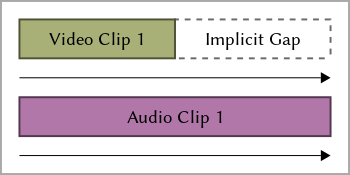
\includegraphics[width=.95\linewidth]{./pics/case1_2.png}
 \caption{Still frames are automatically inserted at implicit gaps to match track duration}
 \label{fig:case1_2}
\end{figure}
You can also add gaps manually, specifying a duration of the gap and inserting it into a video or audio track. The following diagram (figure \ref{fig:case1_3}) shows a parallel with manually added gaps in both video and audio tracks.
\begin{figure}[htbp]
 \centering
 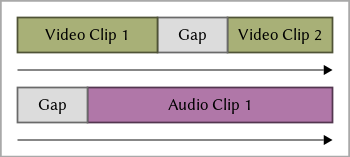
\includegraphics[width=.95\linewidth]{./pics/case1_3.png}
 \caption{Adding explicit gaps manually}
 \label{fig:case1_3}
\end{figure}
Manually added gaps (called \textit{explicit} gaps) are padded with still frames or silence, just as implicit gaps that are added automatically to match track duration.

\subsection{Sequences}

Parallels are put in \textit{sequences}. The parallels within a sequence are played sequentially; the first one is played in its entirety, then the next one, and so on. This behaviour is different from how parallels play their tracks. Parallels and sequences, with their different playback behaviors, make up the fundamental building blocks of the compositional editing in Komposition.

The following diagram (figure \ref{fig:case1_4}) shows a sequence of two parallels, playing sequentially:
\begin{figure}[htbp]
 \centering
 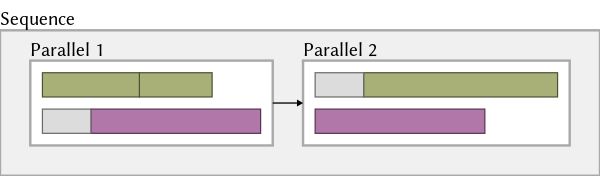
\includegraphics[width=.95\linewidth]{./pics/case1_4.png}
 \caption{A sequence containing two parallels}
 \label{fig:case1_4}
\end{figure}

\subsection{The Timeline}

Finally, at the top level, we have the \textit{timeline}. Effectively, the timeline is a sequence of sequences; it plays every child sequence in sequence. The reason for this level to exist is for the ability to group larger chunks of a screencast within separate sequences.
\begin{figure}[htbp]
 \centering
 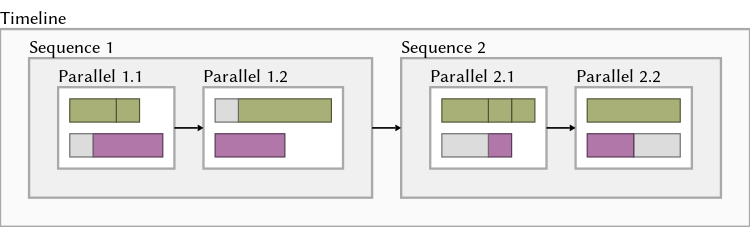
\includegraphics[width=.95\linewidth]{./pics/case1_5.png}
 \caption{A timeline containing two sequences, with two parallels each}
 \label{fig:case1_5}
\end{figure}
I use separate sequences within the timeline to delimit distinct parts of a screencast, such as the introduction, the different chapters, and the summary.


\section{Timeline Flattening}

Komposition currently uses \href{https://ffmpeg.org/}{FFmpeg} to render the final media. This is done by constructing an \texttt{ffmpeg} command invocation with a \href{https://ffmpeg.org/ffmpeg-filters.html}{filter graph} describing how to fit together all clips, still frames, and silent audio parts.

FFmpeg doesn't know about hierarchical timelines; it only cares about video and audio streams. To convert the hierarchical timeline into a suitable representation to build the FFmpeg filter graph from, Komposition performs \textit{timeline flattening}.

The flat representation of a timeline contains only two tracks; audio and video. All gaps are \textit{explicitly} represented in those tracks. The following graph shows how a hierarchical timeline is flattened into two tracks.
\begin{figure}[htbp]
 \centering
 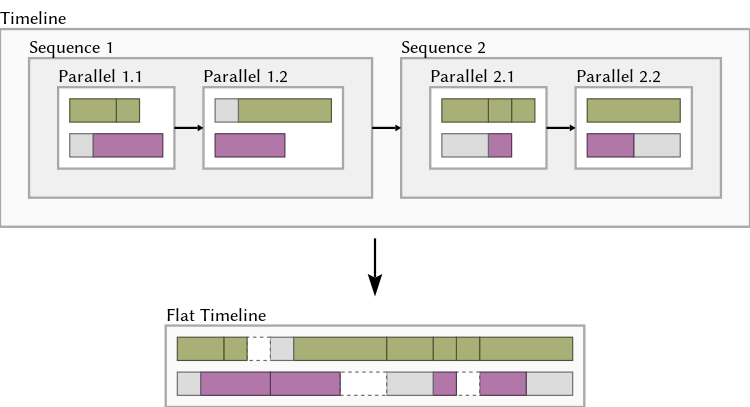
\includegraphics[width=.95\linewidth]{./pics/case1_6.png}
 \caption{Timeline flattening transforming a hierarchical timeline}
 \label{fig:case1_6}
\end{figure}
Notice in the graphic above how the implicit gaps at the ends of video and audio tracks get represented with explicit gaps in the flat timeline. This is because FFmpeg does not know how to render implicit gaps. All gaps are represented explicitly, and are converted to clips of still frames or silent audio when rendered with FFmpeg.

\section{Property Tests}


To test the timeline flattening, there's a number of properties that are checked. I'll go through each one and their property test code.

These properties were primarily written after I already had an implementation. They capture some general properties of flattening that I've come up with. In other cases, I've written properties before beginning on an implementation, or to uncover an existing bug that I've observed.

Thinking about your system's general behaviour and expressing that as executable property tests is hard. I believe, like with any other skill, that it requires a lot of practice. Finding general patterns for properties, like the ones Scott Wlaschin describe in Choosing properties for property-based testing (see chapter \ref{sec:choosing_properties_for_testing}), is a great place to start. When you struggle with finding properties of your system under test, try applying these patterns and see which work for you.



\subsection{Property: Duration Equality}


Given a timeline $t$, where all parallels have at least one video clip, the total duration of the flattened $t$  must be equal to the total duration of $t$. Or, in a more dense notation,

$$\forall t \in T \to duration(flatten(t)) = duration(t)$$

where $T$ is the set of timelines with at least one video clip in each parallel.

The reason that all parallels must have at least one video clip is because currently the flattening algorithm can only locate still frames for video gaps from within the same parallel. If it encounters a parallel with no video clips, the timeline flattening fails. This limitation is discussed in greater detail at the end of this article.

The test for the duration equality property is written using Hedgehog, and looks like this:

\begin{minted}{haskell}
hprop_flat_timeline_has_same_duration_as_hierarchical =
  property $ do
    -- 1. Generate a timeline with video clips in each parallel
    timeline' <- forAll $
        Gen.timeline (Range.exponential 0 5) Gen.parallelWithClips
  
    -- 2. Flatten the timeline and extract the result
    let Just flat = Render.flattenTimeline timeline'
    
    -- 3. Check that hierarchical and flat timeline duration are equal
    durationOf AdjustedDuration timeline'
      === durationOf AdjustedDuration flat
\end{minted}
It generates a timeline using \texttt{forAll} and custom generators (1). Instead of generating timelines of \textit{any} shape and filtering out only the ones with video clips in each parallel, which would be very inefficient, this test uses a custom generator to only obtain inputs that satisfy the invariants of the system under test.

The range passed as the first argument to \texttt{Gen.timeline} is used as the bounds of the generator, such that each level in the generated hierarchical timeline will have at most 5 children.

\texttt{Gen.timeline} takes as its second argument \textit{another generator}, the one used to generate parallels, which in this case is \texttt{Gen.parallelWithClips}. With Hedgehog generators being regular values, it's practical to compose them like this. A ``higher-order generator'' can be a regular function taking other generators as arguments.

As you might have noticed in the assertion (3), \texttt{durationOf} takes as its first argument a value \texttt{AdjustedDuration}. What's that about? Komposition supports adjusting the playback speed of video media for individual clips. To calculate the final duration of a clip, the playback speed needs to taken into account. By passing \texttt{AdjustedDuration} we take playback speed into account for all video clips.

\minisec{SIDETRACK: FINDING A BUG}
Let's say I had introduced a bug in timeline flattening, in which all video gaps weren't added correctly to the flat video tracks. The flattening is implemented as a fold, and it would not be unthinkable that the accumulator was incorrectly constructed in a case. The test would catch this quickly and present us with a minimal counter-example (see figure \ref{fig:case1_7}).
\begin{figure}[htbp]
 \centering
 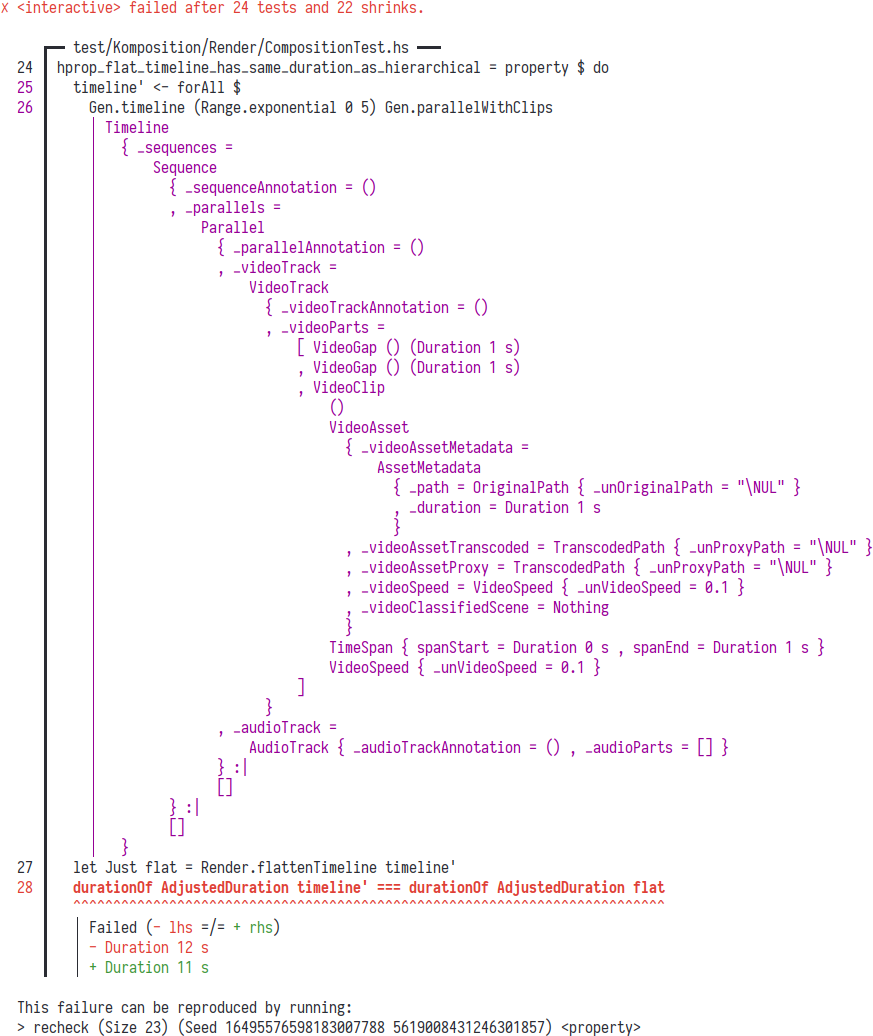
\includegraphics[width=.95\linewidth]{./pics/case1_7.png}
 \caption{Hedgehog presenting a minimal counter-example}
 \label{fig:case1_7}
\end{figure}

Hedgehog prints the source code for the failing property. Below the \texttt{forAll} line the generated value is printed. The difference between the expected and actual value is printed below the failing assertion. In this case it's a simple expression of type \texttt{Duration}. In case you're comparing large tree-like structures, this diff will highlight only the differing expressions. Finally, it prints the following:

This failure can be reproduced by running:
\begin{minted}{haskell}
> recheck (Size 23) (Seed 16495576598183007788 5619008431246301857) <property>
\end{minted}
When working on finding and fixing the fold bug, we can use the printed size and seed values to deterministically rerun the test with the exact same inputs.

\subsection{Property: Clip Occurence}


Slightly more complicated than the duration equality property, the clip occurrence property checks that all clips from the hierarchical timeline, and no other clips, occur within the flat timeline. As discussed in the introduction on timeline flattening, implicit gaps get converted to explicit gaps and thereby add more gaps, but no video or audio clips should be added or removed.

\begin{minted}{haskell}
hprop_flat_timeline_has_same_clips_as_hierarchical =
  property $ do
    -- 1. Generate a timeline with video clips in each parallel
    timeline' <- forAll $
        Gen.timeline (Range.exponential 0 5) Gen.parallelWithClips
    
    -- 2. Flatten the timeline
    let flat = Render.flattenTimeline timeline'
    
    -- 3. Check that all video clips occur in the flat timeline
    flat ^.. _Just . Render.videoParts . each . Render._VideoClipPart
        === timelineVideoClips timeline'
    
    -- 4. Check that all audio clips occur in the flat timeline
    flat ^.. _Just . Render.audioParts . each . Render._AudioClipPart
        === timelineAudioClips timeline'
\end{minted}
The hierarchical timeline is generated and flattened like before (1, 2). The two assertions check that the respective video clips (3) and audio clips (4) are equal. It's using lenses to extract clips from the flat timeline, and the helper functions \texttt{timelineVideoClips} and \texttt{timelineAudioClips} to extract clips from the original hierarchical timeline.


\section{Still Frames Used}

In the process of flattening, the still frame source for each gap is selected. It doesn't assign the actual pixel data to the gap, but a value describing which asset the still frame should be extracted from, and whether to pick the first or the last frame (known as \textit{still frame mode}). This representation lets the flattening algorithm remain a pure function, and thus easier to test. Another processing step runs the effectful action that extracts still frames from video files on disk.

The decision of still frame mode and source is made by the flattening algorithm based on the parallel in which each gap occur, and what video clips are present before or after. It favors using clips occurring after the gap. It only uses frames from clips before the gap in case there are no clips following it. To test this behaviour, I've defined three properties.

\subsection{Property: Single Initial Video Clip}

The following property checks that an initial single video clip, followed by one or more gaps, is used as the still frame source for those gaps.

\begin{minted}{haskell}
hprop_flat_timeline_uses_still_frame_from_single_clip =
  property $ do
    -- 1. Generate a video track generator where the first video part
    --    is always a clip
    let genVideoTrack = do
          v1 <- Gen.videoClip
          vs <- Gen.list (Range.linear 1 5) Gen.videoGap
          pure (VideoTrack () (v1 : vs))
  
    -- 2. Generate a timeline with the custom video track generator
    timeline' <- forAll $ Gen.timeline
      (Range.exponential 0 5)
      (Parallel () <$> genVideoTrack <*> Gen.audioTrack)
  
    -- 3. Flatten the timeline
    let flat = Render.flattenTimeline timeline'
  
    -- 4. Check that any video gaps will use the last frame of a 
    --    preceding video clip
    flat
      ^.. ( _Just
          . Render.videoParts
          . each
          . Render._StillFramePart
          . Render.stillFrameMode
          )
      &   traverse_ (Render.LastFrame ===)
\end{minted}
The custom video track generator (1) always produces tracks with an initial video clip followed by one or more video gaps. The generated timeline (2) can contain parallels with any audio track shape, which may result in a \textit{longer} audio track and thus an implicit gap at the end of the video track. In either case, all video gaps should padded with the last frame of the initial video clip, which is checked in the assertion (4).
\begin{figure}[htbp]
 \centering
 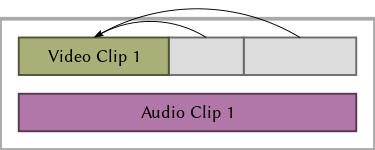
\includegraphics[width=.95\linewidth]{./pics/case1_8.png}
 \caption{Still frames being sourced from the single initial video clip}
 \label{fig:case1_8}
\end{figure}


\subsection{Property: Ending with a Video Clip}


In case the video track ends with a video clip, and is longer than the audio track, all video gaps within the track should use the first frame of a following clip.

\begin{minted}{haskell}
hprop_flat_timeline_uses_still_frames_from_subsequent_clips =
  property $ do
    -- 1. Generate a parallel where the video track ends with a video clip,
    --    and where the audio track is shorter
    let
      genParallel = do
        vt <-
          VideoTrack ()
            <$> (   snoc
                <$> Gen.list (Range.linear 1 10) Gen.videoPart
                <*> Gen.videoClip
                )
        at <- AudioTrack () . pure . AudioGap () <$> Gen.duration'
          (Range.linearFrac
            0
            (durationToSeconds (durationOf AdjustedDuration vt) - 0.1)
          )
        pure (Parallel () vt at)
  
    -- 2. Generate a timeline with the custom parallel generator
    timeline' <- forAll $ Gen.timeline (Range.exponential 0 5) genParallel
  
    -- 3. Flatten the timeline
    let flat = Render.flattenTimeline timeline'
  
    -- 4. Check that all gaps use the first frame of subsequent clips
    flat
      ^.. ( _Just
          . Render.videoParts
          . each
          . Render._StillFramePart
          . Render.stillFrameMode
          )
      &   traverse_ (Render.FirstFrame ===)
\end{minted}
The custom generator (1) produces parallels where the video track is guaranteed to end with a clip, and where the audio track is 100 ms shorter than the video track. This ensures that there's no implicit video gap at the end of the video track. Generating (2) and flattening (3) is otherwise the same as before. The assertion (4) checks that all video gaps uses the first frame of a following clip.
\begin{figure}[htbp]
 \centering
 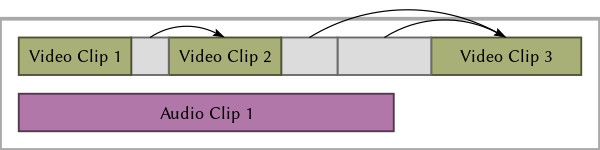
\includegraphics[width=.95\linewidth]{./pics/case1_9.png}
 \caption{Still frames being sourced from following video clips when possible}
 \label{fig:case1_9}
\end{figure}


\subsection{Property: Ending with an Implicit Video Gap}


The last property on still frame usage covers the case where the video track is shorter than the audio track. This leaves an implicit gap which, just like explicit gaps inserted by the user, are padded with still frames.

\begin{minted}{haskell}
hprop_flat_timeline_uses_last_frame_for_automatic_video_padding =
  property $ do
    -- 1. Generate a parallel where the video track only contains a video
    --    clip, and where the audio track is longer
    let
      genParallel = do
        vt <- VideoTrack () . pure <$> Gen.videoClip
        at <- AudioTrack () . pure . AudioGap () <$> Gen.duration'
          (Range.linearFrac
            (durationToSeconds (durationOf AdjustedDuration vt) + 0.1)
            10
          )
        pure (Parallel () vt at)
  
    -- 2. Generate a timeline with the custom parallel generator
    timeline' <- forAll $ Gen.timeline (Range.exponential 0 5) genParallel
  
    -- 3. Flatten the timeline
    let flat = Render.flattenTimeline timeline'
  
    -- 4. Check that video gaps (which should be a single gap at the
    --    end of the video track) use the last frame of preceding clips
    flat
      ^.. ( _Just
          . Render.videoParts
          . each
          . Render._StillFramePart
          . Render.stillFrameMode
          )
      &   traverse_ (Render.LastFrame ===)
\end{minted}
The custom generator (1) generates a video track consisting of video clips only, and an audio track that is 100ms longer. Generating the timeline (2) and flattening (3) are again similar to the previous property tests. The assertion (4) checks that all video gaps use the last frame of preceding clips, even if we know that there should only be one at the end.
\begin{figure}[htbp]
 \centering
 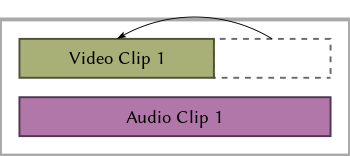
\includegraphics[width=.95\linewidth]{./pics/case1_10.png}
 \caption{Still frames being sourced from preceding video clip for last implicit gap}
 \label{fig:case1_10}
\end{figure}



\section{Properties: Flattening Equivalences}

The last property I want to show in this case study checks flattening at the sequence and parallel levels. While rendering a full project always flattens at the timeline, the \textit{preview} feature in Komposition can be used to render and preview a single sequence or parallel.

There should be no difference between flattening an entire timeline and flattening all of its sequences or parallels and folding those results into a single flat timeline. This is what the \textit{flattening equivalences} properties are about.

\begin{minted}{haskell}
hprop_flat_timeline_is_same_as_all_its_flat_sequences =
  property $ do
    -- 1. Generate a timeline
    timeline' <- forAll $
      Gen.timeline (Range.exponential 0 5) Gen.parallelWithClips
  
    -- 2. Flatten all sequences and fold the resulting flat
    --    timelines together
    let flat = timeline' ^.. sequences . each
               & foldMap Render.flattenSequence
  
    -- 3. Make sure we successfully flattened the timeline
    flat /== Nothing
               
    -- 4. Flatten the entire timeline and compare to the flattened 
    --    sequences
    Render.flattenTimeline timeline' === flat
\end{minted}
The first property generates a timeline (1) where all parallels have at least one video clip. It flattens all sequences within the timeline and folds the results together (2). Folding flat timelines together means concatenating their video and audio tracks, resulting in a single flat timeline.

Before the final assertion, it checks that we got a result (3) and not Nothing. As it's using the \texttt{Gen.parallelWithClips} generator there should always be video clips in each parallel, and we should always successfully flatten and get a result. The final assertion (4) checks that rendering the original timeline gives the same result as the folded-together results of rendering each sequence.

The other property is very similar, but operates on parallels rather than sequences:

\begin{minted}{haskell}
hprop_flat_timeline_is_same_as_all_its_flat_parallels =
  property $ do
    -- 1. Generate a timeline
    timeline' <- forAll $
      Gen.timeline (Range.exponential 0 5) Gen.parallelWithClips
  
    -- 2. Flatten all parallels and fold the resulting flat
    --    timelines together
    let flat = timeline' ^.. sequences . each . parallels . each
               & foldMap Render.flattenParallel
  
    -- 3. Make sure we successfully flattened the timeline
    flat /== Nothing
  
    -- 4. Flatten the entire timeline and compare to the flattened 
    --    parallels
    Render.flattenTimeline timeline' === flat
\end{minted}
The only difference is in the traversal (2), where we apply \texttt{Render.flattenParallel} to each parallel instead of applying \texttt{Render.flattenSequence} to each sequence.


\section{Missing Properties}

Whew! That was quite a lot of properties and code, especially for a warm-up. But timeline flattening could be tested more thoroughly! I haven't yet written the following properties, but I'm hoping to find some time to add them:

\begin{itemize}
\item \textbf{Clip playback timestamps are the same}. The ``clip occurrence'' property only checks that the hierarchical timeline's clips occur in the flat timeline. It doesn't check when in the flat timeline they occur. One way to test this would be to first annotate each clip in original timeline with its playback timestamp, and transfer this information through to the flat timeline. Then the timestamps could be included in the assertion.

\item \textbf{Source assets used as still frame sources}. The ``still frames used'' properties only check the still frame mode of gaps, not the still frame sources. The algorithm could have a bug where it always uses the first video clip's asset as a frame source, and the current property tests would not catch it.

\item \textbf{Same flat result is produced regardless of sequence grouping}. Sequences can be split or joined in any way without affecting the final rendered media. They are merely ways of organizing parallels in logical groups. A property could check that however you split or join sequences within a timeline, the flattened result is the same.
\end{itemize}

\section{A Missing Feature}

As pointed out earlier, parallels must have at least one video clip. The flattening algorithm can only locate still frame sources for video gaps from within the same parallel. This is an annoying limitation when working with Komposition, and the algorithm should be improved.

As the existing set of properties describe timeline flattening fairly well, changing the algorithm could be done with a TDD-like workflow:

\begin{enumerate}
\item Modify the property tests to capture the intended behaviour
\item Tests will fail, with the errors showing how the existing implementation fails to find still frame sources as expected
\item Change the implementation to make the tests pass                                                
\end{enumerate}
PBT is not only an after-the-fact testing technique. It can be used much like conventional example-based testing to drive development.

\section{Obligatory Cliff-Hanger}

In this post we've looked at timeline flattening, the simplest case study in the ``Property-Based Testing in a Screencast Editor'' series. The system under test was a module of pure functions, with complex enough behaviour to showcase PBT as a valuable tool. The tests are more closely related to the design choices and concrete representations of the implementation.

Coming case studies will dive deeper into the more complex subsystems of Komposition, and finally we'll see how PBT can be used for integration testing. At that level, the property tests are less tied to the implementation, and focus on describing the higher-level outcomes of the interaction between subsystems.

Next up is property tests for the video classifier. It's also implemented a pure function, but with slightly more complicated logic that is trickier to test. We're going to look at an interesting technique where we generate the \textit{expected output} instead of the input.



\chapter{Case Study 2: Video Scene Classification - Oskar Wickstr\"om}
\label{sec:video_scene_classification}

\vspace{\baselineskip}
\noindent\textit{Original article: \cite{video_scene_classification}}
\vspace{\baselineskip}

\noindent In the last case study on property-based testing (PBT) in Komposition we looked at timeline flattening. This post covers the video classifier, how it was tested before, and the bugs I found when I wrote property tests for it.

If you haven't read the introduction (see \ref{sec:screencast_introduction}) or the first case study (see \ref{sec:timeline_flattening}) yet, I recommend checking them out!

\section{Classifying Scenes in Imported Video}


Komposition can automatically classify \textit{scenes} when importing video files. This is a central productivity feature in the application, effectively cutting recorded screencast material automatically, letting the user focus on arranging the scenes of their screencast. Scenes are segments that are considered \textit{moving}, as opposed to \textit{still} segments:

\begin{itemize}
\item A still segment is a sequence of at least $S$ seconds of \textit{near-equal} frames
\item A moving segment is a sequence of \textit{non-equal} frames, or a sequence of near-equal frames with a duration less than $S$
\end{itemize}
$S$ is a preconfigured minimum still segment duration in Komposition. In the future it might be configurable from the user interface, but for now it's hard-coded.

Equality of two frames $f_1$ and $f_2$ is defined as a function $E(f_1,f_2)$, described informally as:

\begin{itemize}
\item comparing corresponding pixel color values of $f_1$  and $f_2$, with a small epsilon for tolerance of color variation, and
\item deciding two frames equal when at least 99\% of corresponding pixel pairs are considered equal.                                                                                              \end{itemize}
In addition to the rules stated above, there are two edge cases:

\begin{enumerate}
\item The first segment is always a considered a moving segment (even if it's just a single frame)
\item The last segment may be a still segment with a duration less than $S$
\end{enumerate}
The second edge case is not what I would call a desirable feature, but rather a shortcoming due to the classifier not doing any type of backtracking. This could be changed in the future.

\section{Manually Testing the Classifier}


The first version of the video classifier had no property tests. Instead, I wrote what I thought was a decent classifier algorithm, mostly messing around with various pixel buffer representations and parallel processing to achieve acceptable performance.

The only type of testing I had available, except for general use of the application, was a color-tinting utility. This was a separate program using the same classifier algorithm. It took as input a video file, and produced as output a video file where each frame was tinted green or red, for moving and still frames, respectively (Note from the editor: on the web-page there is a GIF showing the color tinting. For obvious reasons, an anmiated GIF cannot be included here).

In the (in this document omitted) recording above you see the color-tinted output video based on a recent version of the classifier. It classifies moving and still segments rather accurately. Before I wrote property tests and fixed the bugs that I found, it did not look so pretty, flipping back and forth at seemingly random places.

At first, debugging the classifier with the color-tinting tool way seemed like a creative and powerful technique. But the feedback loop was horrible, having to record video, process it using the slow color-tinting program, and inspecting it by eye. In hindsight, I can conclude that PBT is far more effective for testing the classifier.

\section{Video Classification Properties}


Figuring out how to write property tests for video classification wasn't obvious to me. It's not uncommon in example-based testing that tests end up mirroring the structure, and even the full implementation complexity, of the system under test. The same can happen in property-based testing.

With some complex systems it's very hard to describe the correctness as a relation between any valid input and the system's observed output. The video classifier is one such case. How do I decide if an output classification is correct for a specific input, without reimplementing the classification itself in my tests?

The other way around is easy, though! If I have a classification, I can convert that into video frames. Thus, the solution to the testing problem is to not generate the input, but instead generate the expected output. Hillel Wayne calls this technique ``oracle generators'' in his recent article\footnote{See the ``Oracle Generators'' section in Finding Property Tests (see \ref{sec:finding_property_tests}).}.

The classifier property tests generate high-level representations of the expected classification output, which are lists of values describing the type and duration of segments.
\begin{figure}[htbp]
 \centering
 
\includegraphics[width=.95\linewidth]{./pics/case2_1.png}
 \caption{A generated sequence of expected classified segments}
 \label{fig:case2_1}
\end{figure}
Next, the list of output segments is converted into a sequence of actual frames. Frames are two-dimensional arrays of RGB pixel values. The conversion is simple:

\begin{itemize}
\item Moving segments are converted to a sequence of alternating frames, flipping between all gray and all white pixels
\item Still frames are converted to a sequence of frames containing all black pixels
\end{itemize}
The example sequence in the diagram above, when converted to pixel frames with a frame rate of 10 FPS, can be visualized like in the following diagram, where each thin rectangle represents a frame:
\begin{figure}[htbp]
 \centering
 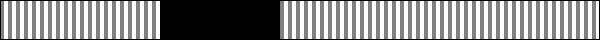
\includegraphics[width=.95\linewidth]{./pics/case2_2.png}
 \caption{Pixel frames derived from a sequence of expected classified output segments}
 \label{fig:case2_2}
\end{figure}
By generating high-level output and converting it to pixel frames, I have input to feed the classifier with, and I know what output it should produce. Writing effective property tests then comes down to writing generators that produce valid output, according to the specification of the classifier. In this post I'll show two such property tests.

\section{Testing Still Segment Minimum Length}

As stated in the beginning of this post, classified still segments must have a duration greater than or equal to $S$
, where $S$ is the minimum still segment duration used as a parameter for the classifier. The first property test we'll look at asserts that this invariant holds for all classification output.

\begin{minted}{haskell}
hprop_classifies_still_segments_of_min_length = property $ do

  -- 1. Generate a minimum still segment length/duration
  minStillSegmentFrames <- forAll $ Gen.int (Range.linear 2 (2 * frameRate))
  let minStillSegmentTime = frameCountDuration minStillSegmentFrames

  -- 2. Generate output segments
  segments <- forAll $
    genSegments (Range.linear 1 10)
                (Range.linear 1
                              (minStillSegmentFrames * 2))
                (Range.linear minStillSegmentFrames
                              (minStillSegmentFrames * 2))
                resolution

  -- 3. Convert test segments to actual pixel frames
  let pixelFrames = testSegmentsToPixelFrames segments

  -- 4. Run the classifier on the pixel frames
  let counted = classifyMovement minStillSegmentTime (Pipes.each pixelFrames)
                & Pipes.toList
                & countSegments

  -- 5. Sanity check
  countTestSegmentFrames segments === totalClassifiedFrames counted

  -- 6. Ignore last segment and verify all other segments
  case initMay counted of
    Just rest ->
      traverse_ (assertStillLengthAtLeast minStillSegmentTime) rest
    Nothing -> success
  where
    resolution = 10 :. 10
\end{minted}
This chunk of test code is pretty busy, and it's using a few helper functions that I'm not going to bore you with. At a high level, this test:

\begin{enumerate}
\item Generates a minimum still segment duration, based on a minimum frame count (let's call it $n$) in the range 
$[2,20]$. The classifier currently requires that $n \geq 2$, hence the lower bound. The upper bound of 20 frames is an arbitrary number that I've chosen.
\item Generates valid output segments using the custom generator \texttt{genSegments}, where
\begin{itemize}
\item moving segments have a frame count in $[1,2n]$, and
\item still segments have a frame count in $[n,2n]$.
\end{itemize}
\item Converts the generated output segments to actual pixel frames. This is done using a helper function that returns a list of alternating gray and white frames, or all black frames, as described earlier.
\item Count the number of consecutive frames within each segment, producing a list like \texttt{[Moving 18, Still 5, Moving 12, Still 30]}.
\item Performs a sanity check that the number of frames in the generated expected output is equal to the number of frames in the classified output. The classifier must not lose or duplicate frames.
\item Drops the last classified segment, which according to the specification can have a frame count less than $n$, and asserts that all other still segments have a frame count greater than or equal to $n$. 
\end{enumerate}
Let's run some tests.

\begin{minted}{haskell}
> :{
| hprop_classifies_still_segments_of_min_length
|   & Hedgehog.withTests 10000
|   & Hedgehog.check
| :}
\end{minted}
\texttt{  \checkmark <interactive> passed 10000 tests.}\\
Cool, it looks like it's working.

\minisec{Sidetrack: Why generate the output?}

Now, you might wonder why I generate output segments first, and then convert to pixel frames. Why not generate random pixel frames to begin with? The property test above only checks that the still segments are long enough!

The benefit of generating valid output becomes clearer in the next property test, where I use it as the expected output of the classifier. Converting the output to a sequence of pixel frames is easy, and I don't have to state any complex relation between the input and output in my property. When using oracle generators, the assertions can often be plain equality checks on generated and actual output.

But there's benefit in using the same oracle generator for the ``minimum still segment length'' property, even if it's more subtle. By generating valid output and converting to pixel frames, I can generate inputs that cover the edge cases of the system under test. Using property test statistics and coverage checks, I could inspect coverage, and even fail test runs where the generators don't hit enough of the cases I'm interested in\footnote{John Hughes' talk \href{https://www.youtube.com/watch?v=NcJOiQlzlXQ}{Building on developers' intuitions} goes into depth on this. There's also \href{https://github.com/hedgehogqa/haskell-hedgehog/pull/253}{work being done} to provide similar functionality for Hedgehog.}.

Had I generated random sequences of pixel frames, then perhaps the majority of the generated examples would only produce moving segments. I could tweak the generator to get closer to either moving or still frames, within some distribution, but wouldn't that just be a variation of generating valid scenes? It would be worse, in fact. I wouldn't then be reusing existing generators, and I wouldn't have a high-level representation that I could easily convert from and compare with in assertions.


\section{Testing Moving Segment Time Spans}


The second property states that the classified moving segments must start and end at the same timestamps as the moving segments in the generated output. Compared to the previous property, the relation between generated output and actual classified output is stronger.

\begin{minted}{haskell}
hprop_classifies_same_scenes_as_input = property $ do
  -- 1. Generate a minimum still still segment duration
  minStillSegmentFrames <- forAll $ Gen.int (Range.linear 2 (2 * frameRate))
  let minStillSegmentTime = frameCountDuration minStillSegmentFrames

  -- 2. Generate test segments
  segments <- forAll $ genSegments (Range.linear 1 10)
                                   (Range.linear 1
                                                 (minStillSegmentFrames * 2))
                                   (Range.linear minStillSegmentFrames
                                                 (minStillSegmentFrames * 2))
                                   resolution

  -- 3. Convert test segments to actual pixel frames
  let pixelFrames = testSegmentsToPixelFrames segments

  -- 4. Convert expected output segments to a list of expected time spans
  --    and the full duration
  let durations = map segmentWithDuration segments
      expectedSegments = movingSceneTimeSpans durations
      fullDuration = foldMap unwrapSegment durations

  -- 5. Classify movement of frames
  let classifiedFrames =
        Pipes.each pixelFrames
        & classifyMovement minStillSegmentTime
        & Pipes.toList

  -- 6. Classify moving scene time spans
  let classified =
        (Pipes.each classifiedFrames
         & classifyMovingScenes fullDuration)
        >-> Pipes.drain
        & Pipes.runEffect
        & runIdentity

  -- 7. Check classified time span equivalence
  expectedSegments === classified

  where
    resolution = 10 :. 10
\end{minted}
Steps 1--3 are the same as in the previous property test. From there, this test:

\begin{description}
\item [4.] Converts the generated output segments into a list of time spans. Each time span marks the start and end of an expected moving segment. Furthermore, it needs the full duration of the input in step 6, so that's computed here.
\item [5.] Classify the movement of each frame, i.e. if it's part of a moving or still segment.
\item [6.]Run the second classifier function called classifyMovingScenes, based on the full duration and the frames with classified movement data, resulting in a list of time spans.
\item [7.] Compare the expected and actual classified list of time spans.
\end{description}
While this test looks somewhat complicated with its setup and various conversions, the core idea is simple. But is it effective?



\section{Bugs! Bugs everywhere!}

Preparing for a talk on property-based testing, I added the ``moving segment time spans'' property a week or so before the event. At this time, I had used Komposition to edit multiple screencasts. Surely, all significant bugs were caught already. Adding property tests should only confirm the level of quality the application already had. Right?

Nope. First, I discovered that my existing tests were fundamentally incorrect to begin with. They were not reflecting the specification I had in mind, the one I described in the beginning of this post.

Furthermore, I found that the generators had errors. At first, I used Hedgehog to generate the pixels used for the classifier input. Moving frames were based on a majority of randomly colored pixels and a small percentage of equally colored pixels. Still frames were based on a random single color.

The problem I had not anticipated was that the colors used in moving frames were not guaranteed to be distinct from the color used in still frames. In small-sized examples I got black frames at the beginning and end of moving segments, and black frames for still segments, resulting in different classified output than expected. Hedgehog shrinking the failing examples' colors towards 0, which is black, highlighted this problem even more.

I made my generators much simpler, using the alternating white/gray frames approach described earlier, and went on to running my new shiny tests. Here's what I got:
\begin{figure}[htbp]
 \centering
 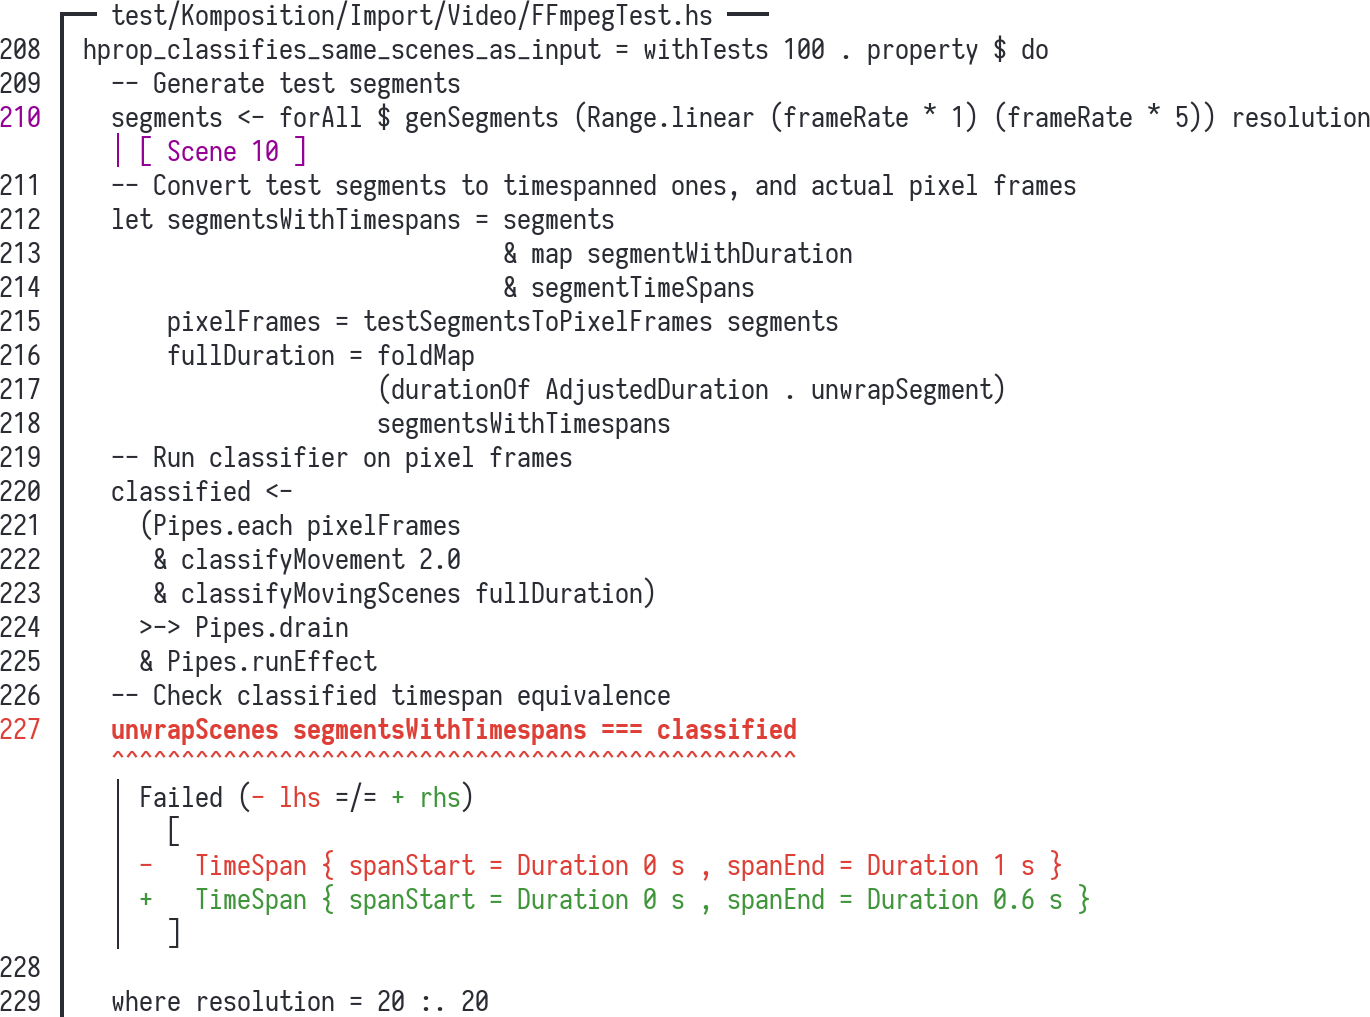
\includegraphics[width=.95\linewidth]{./pics/case2_3.png}
 \caption{Hedgehog output}
 \label{fig:case2_3}
\end{figure}
What? Where does 0s--0.6s come from? The classified time span should've been 0s--1s, as the generated output has a single moving scene of 10 frames (1 second at 10 FPS). I started digging, using the \texttt{annotate} function in Hedgehog to inspect the generated and intermediate values in failing examples.

I couldn't find anything incorrect in the generated data, so I shifted focus to the implementation code. The end timestamp 0.6s was consistently showing up in failing examples. Looking at the code, I found a curious hard-coded value 0.5 being bound and used locally in \texttt{classifyMovement}.

The function is essentially a \textit{fold} over a stream of frames, where the accumulator holds vectors of previously seen and not-yet-classified frames. Stripping down and simplifying the old code to highlight one of the bugs, it looked something like this:

\begin{minted}{haskell}
classifyMovement minStillSegmentTime =
  case ... of
    InStillState{..} ->
      if someDiff > minEqualTimeForStill
        then ...
        else ...
    InMovingState{..} ->
      if someOtherDiff >= minStillSegmentTime
        then ...
        else ...
  where
    minEqualTimeForStill = 0.5
\end{minted}
Let's look at what's going on here. In the \texttt{InStillState} branch it uses the value \texttt{minEqualTimeForStill}, instead of always using the \texttt{minStillSegmentTime} argument. This is likely a residue from some refactoring where I meant to make the value a parameter instead of having it hard-coded in the definition.

Sparing you the gory implementation details, I'll outline two more problems that I found. In addition to using the hard-coded value, it incorrectly classified frames based on that value. Frames that should've been classified as ``moving'' ended up ``still''. That's why I didn't get 0s--1s in the output.

Why didn't I see 0s--0.5s, given the hard-coded value 0.5? Well, there was also an off-by-one bug, in which one frame was classified incorrectly together with the accumulated moving frames.

The \texttt{classifyMovement} function is 30 lines of Haskell code juggling some state, and I managed to mess it up in three separate ways at the same time. With these tests in place I quickly found the bugs and fixed them. I ran thousands of tests, all passing.

Finally, I ran the application, imported a previously recorded video, and edited a short screencast. The classified moving segments where \textit{notably} better than before.

\section{Summary}


A simple streaming fold can hide bugs that are hard to detect with manual testing. The consistent result of 0.6, together with the hard-coded value 0.5 and a frame rate of 10 FPS, pointed clearly towards an off-by-one bug. I consider this is a great showcase of how powerful shrinking in PBT is, consistently presenting minimal examples that point towards specific problems. It's not just a party trick on ideal mathematical functions.

Could these errors have been caught without PBT? I think so, but what effort would it require? Manual testing and introspection did not work for me. Code review might have revealed the incorrect definition of \texttt{minEqualTimeForStill}, but perhaps not the off-by-one and incorrect state handling bugs. There are of course many other QA techniques, I won't evaluate all. But given the low effort that PBT requires in this setting, the amount of problems it finds, and the accuracy it provides when troubleshooting, I think it's a clear win.

I also want to highlight the iterative process that I find naturally emerges when applying PBT:

\begin{enumerate}
\item Think about how your system is supposed to work. Write down your specification.
\item Think about how to generate input data and how to test your system, based on your specification. Tune your generators to provide better test data. Try out alternative styles of properties. Perhaps model-based or metamorphic testing fits your system better.
\item Run tests and analyze the minimal failing examples. Fix your implementation until all tests pass.
\end{enumerate}
This can be done when modifying existing code, or when writing new code. You can apply this without having any implementation code yet, perhaps just a minimal stub, and the workflow is essentially the same as TDD.

\section{Coming Up}

The final post in this series will cover testing at a higher level of the system, with effects and multiple subsystems being integrated to form a full application. We will look at property tests that found many bugs and that made a substantial refactoring possible.




\chapter{Case Study 3: Integration Testing - Oskar Wickstr\"om}
\label{sec:integration_testing}

\vspace{\baselineskip}
\noindent\textit{Original article: \cite{integration_testing}}
\vspace{\baselineskip}

\noindent This is the final case study in the ``Property-Based Testing in a Screencast Editor'' series. It covers property-based integration testing and its value during aggressive refactoring work within Komposition.

\section{A History of Two Stacks}


In Komposition, a project's state is represented using an in-memory data structure. It contains the hierarchical timeline, the focus, import and render settings, project storage file paths, and more. To let users navigate backwards and forwards in their history of project edits, for example when they have made a mistake, Komposition supplies \textit{undo} and \textit{redo} commands.

The undo/redo history was previously implemented as a data structure recording project states, compromised of:

\begin{itemize}
\item a \textit{current state} variable
\item a stack of \textit{previous states}
\item a stack of \textit{possible future states}
\end{itemize}
The undo/redo history data structure held entire project state values. Each undoable and redoable user action created a new state value. Let's look a bit closer at how this worked.

\subsection{Performing Actions}


When a user performed an undoable/redoable action, the undo/redo history would:

\begin{itemize}
\item push the previous state onto the undo stack
\item perform the action and replace the current state
\item discard all states in the redo stack
\end{itemize}
This can be visualized as in the following diagram, where the state $d$ is being replaced with a new state $h$, and $d$ being pushed onto the undo stack. The undo/redo history to the left of the dividing line is the original, and the one to the right is the resulting history.
\begin{figure}[htbp]
 \centering
 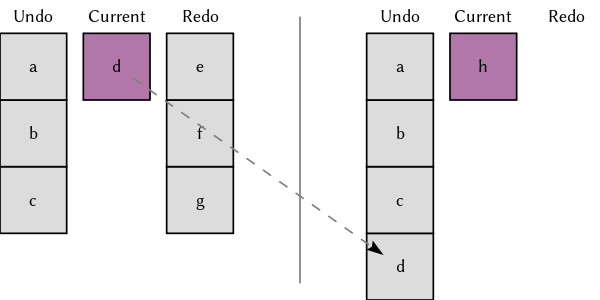
\includegraphics[width=.95\linewidth]{./pics/case3_1.png}
 \caption{Performing an action pushes the previous state onto the undo stack and discards the redo stack}
 \label{fig:case3_1}
\end{figure}
Again, note that performing new actions discarded all states in the redo stack.

\subsection{Undoing Actions}

When the user chose to undo an action, the undo/redo history would:

\begin{itemize}
\item pop the undo stack and use that state as the current state
\item push the previous state onto the redo stack
\end{itemize}
The following diagram shows how undoing the last performed action's resulting state, $d$, pushes $d$ onto the redo stack, and pops $c$ from the undo stack to use that as the current state.
\begin{figure}[htbp]
 \centering
 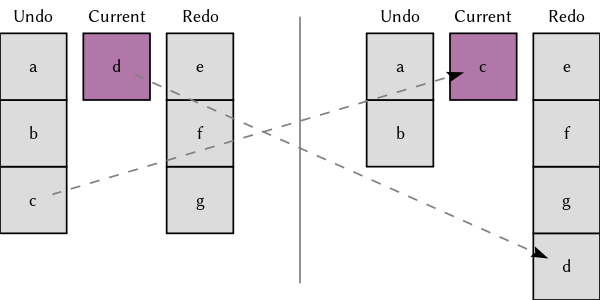
\includegraphics[width=.95\linewidth]{./pics/case3_2.png}
 \caption{Undoing pushes the previous state onto the redo stack and pops the undo stack for a current state}
 \label{fig:case3_2}
\end{figure}

\subsection{Redoing Actions}


When the user chose to redo an action, the undo/redo history would:

\begin{itemize}
\item pop the redo stack and use that state as the current state
\item push the previous state onto the undo stack
\end{itemize}
The last diagram shows how redoing, recovering a previously undone state, pops g from the redo stack to use that as the current state, and pushes the previous state d onto the undo stack.
\begin{figure}[htbp]
 \centering
 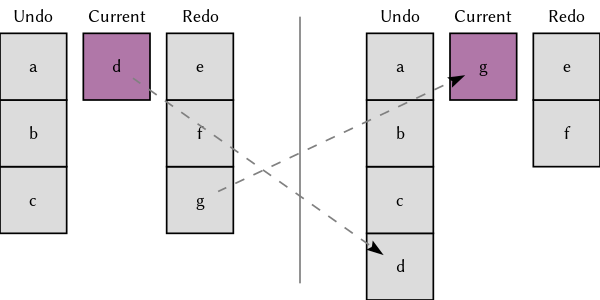
\includegraphics[width=.95\linewidth]{./pics/case3_3.png}
 \caption{Undoing pushes the previous state onto the redo stack and pops the undo stack for a current state}
 \label{fig:case3_3}
\end{figure}
Note that not all user actions in Komposition are undoable/redoable. Actions like navigating the focus or zooming are not recorded in the history.


\subsection{Dealing With Performance Problems}

While the ``two stacks of states'' algorithm was easy to understand and implement, it failed to meet my non-functional requirements. A screencast project compromised of hundreds or thousands of small edits would consume gigabytes of disk space when stored, take tens of seconds to load from disk, and consume many gigabytes of RAM when in memory.

Now, you might think that my implementation was incredibly naive, and that the performance problems could be fixed with careful profiling and optimization. And you'd probably be right! I did consider going down that route, optimizing the code, time-windowing edits to compact history on the fly, and capping the history at some fixed size. Those would all be interesting pursuits, but in the end I decided to try something else.


\section{Refactoring with Property-Based Integration Tests}


Instead of optimizing the current stack-based implementation, I decided to implement the undo/redo history in terms of \href{https://en.wikipedia.org/wiki/Inverse_function}{inverse actions}. In this model, actions not only modify the project state, they also return another action, its inverse, that \textit{reverses} the effects of the original action. Instead of recording a new project state data structure for each edit, the history only records descriptions of the actions themselves.

I realized early that introducing the new undo/redo history implementation in Komposition was not going to be a small task. It would touch the majority of command implementation code, large parts of the main application logic, and the project binary serialization format. What it wouldn't affect, though, was the module describing user commands in abstract.

To provide a safety net for the refactoring, I decided to cover the undo/redo functionality with tests. As the user commands would stay the same throughout my modifications, I chose to test at that level, which can be characterized as integration-level testing. The tests run Komposition, including its top-level application control flow, but with the user interface and some other effects stubbed out. Making your application testable at this level is hard work, but the payoff can be huge.

With Komposition featuring close to twenty types of user commands, combined with a complex hierarchical timeline and navigation model, the combinatory explosion of possible states was daunting. Relying on example-based tests to safeguard my work was not satisfactory. While PBT couldn't cover the entire state space either, I was confident it would improve my chances of finding actual bugs.


\subsection{Undo/Redo Tests}


Before I began refactoring, I added tests for the inverse property of undoable/redoable actions. The first test focuses on undoing actions, and is structured as follows:

\begin{enumerate}
\item Generate an initial project and application state
\item Generate a sequence of undoable/redoable commands (wrapped in \textit{events})
\item Run the application with the initial state and the generated events
\item Run an undo command for each original command
\item Assert that final timeline is equal to the initial timeline
\end{enumerate}
Let's look at the Haskell Hedgehog property test:

\begin{minted}{haskell}
hprop_undo_actions_are_undoable = property $ do

  -- 1. Generate initial timeline and focus
  timelineAndFocus <- forAllWith showTimelineAndFocus $
    Gen.timelineWithFocus (Range.linear 0 10) Gen.parallel

  -- ... and initial application state
  initialState <- forAll (initializeState timelineAndFocus)

  -- 2. Generate a sequence of undoable/redoable commands
  events <- forAll $
    Gen.list (Range.exponential 1 100) genUndoableTimelineEvent

  -- 3. Run 'events' on the original state
  beforeUndos <- runTimelineStubbedWithExit events initialState

  -- 4. Run as many undo commands as undoable commands
  afterUndos <- runTimelineStubbedWithExit (undoEvent <$ events) beforeUndos

  -- 5. That should result in a timeline equal to the one we started
  -- with
  timelineToTree (initialState ^. currentTimeline)
    === timelineToTree (afterUndos ^. currentTimeline)
\end{minted}
The second test, focusing on redoing actions, is structured very similarly to the previous test:

\begin{enumerate}
\item Generate an initial project and application state
\item Generate a sequence of undoable commands (wrapped in \textit{events})
\item Run the application with the initial state and the generated events
\item Run an undo commands for each original command
\item Run an redo commands for each original command
\item Assert that final timeline is equal to the timeline before undoing actions
\end{enumerate}
The test code is also very similar:

\begin{minted}{haskell}
hprop_undo_actions_are_redoable = property $ do

  -- 1. Generate the initial timeline and focus
  timelineAndFocus <- forAllWith showTimelineAndFocus $
    Gen.timelineWithFocus (Range.linear 0 10) Gen.parallel

  -- ... and the initial application state
  initialState <- forAll (initializeState timelineAndFocus)

  -- 2. Generate a sequence of undoable/redoable commands
  events <- forAll $
    Gen.list (Range.exponential 1 100) genUndoableTimelineEvent

  -- 3. Run 'events' on the original state
  beforeUndos <- runTimelineStubbedWithExit events initialState

  -- 4. Run undo commands corresponding to all original commands
  afterRedos  <-
    runTimelineStubbedWithExit (undoEvent <$ events) beforeUndos
    -- 5. Run redo commands corresponding to all original commands
    >>= runTimelineStubbedWithExit (redoEvent <$ events)

  -- 6. That should result in a timeline equal to the one we had
  -- before undoing actions
  timelineToTree (beforeUndos ^. currentTimeline)
    === timelineToTree (afterRedos ^. currentTimeline)
\end{minted}
Note that these tests only assert on the equality of timelines, not entire project states, as undoable commands only operate on the timeline.

\subsection{All Tests Passing, Everything Works}


The undo/redo tests were written and run on the original stack-based implementation, kept around during a refactoring that took me two weeks of hacking during late nights and weekends, and finally run and passing with the new implementation based on inverse actions. Except for a few minimal adjustments to data types, these tests stayed untouched during the entire process.

The confidence I had when refactoring felt like a super power. Two simple property tests made the undertaking possible. They found numerous bugs, including:

\begin{itemize}
\item Off-by-one index errors in actions modifying the timeline
\item Inconsistent timeline focus:
    \begin{itemize}
    \item focus was incorrectly restored on undoing an action
    \item focus was outside of the timeline bounds
    \end{itemize}
\item Non-inverse actions:
    \begin{itemize}
    \item actions returning incorrectly constructed inverses
    \item the inverse of splitting a sequence is joining sequences, and joining them back up didn't always work
    \end{itemize}
\end{itemize}
After all tests passed, I ran the application with its GUI, edited a screencast project, and it all worked flawlessly. It's almost too good to be true, right?

Property testing is not a silver bullet, and there might still be bugs lurking in my undo/redo history implementation. The tests I run are never going to be exhaustive and my generators might be flawed. That being said, they gave me a confidence in refactoring that I've never had before. Or maybe I just haven't hit that disastrous edge case yet?

\section{Why Test With Properties?}
This was the last case study in the ``Property-Based Testing in a Screencast Editor'' series. I've had a great time writing these articles and giving talks on the subject. Before I wrap up, I'll summarize my thoughts on PBT in general and my experience with it in Komposition.

Property-based testing is not only for pure functions; you can use it to test effectful actions. It is not only for unit testing; you can write integration tests using properties. It's not only for functional programming languages; there are good frameworks for most popular programming languages.

Properties describe the general behavior of the system under test, and verify its correctness using a variety of inputs. Not only is this an effective way of finding errors, it's also a concise way of documenting the system.

The iterative process in property-based testing, in my experience, comes down to the following steps:

\begin{enumerate}
\item Think about the specification of your system under test
\item Think about how generators and tests should work
\item Write or modify generators, tests, and implementation code, based on steps 1 and 2
\item Get minimal examples of failing tests
\item Repeat
\end{enumerate}
Using PBT within Komposition has made it possible to confidently refactor large parts of the application. It has found errors in my thinking, my generators, my tests, and in my implementation code. Testing video scene classification went from a time consuming, repetitive, and manual verification process to a fast, effective, and automated task.

In short, it's been a joy, and I look forward to continue using PBT in my work and in my own projects. I hope I've convinced you of its value, and inspired you to try it out, no matter what kind of project you're working on and what programming language you are using. Involve your colleagues, practice writing property tests together, and enjoy finding complicated bugs before your users do!
